 
\chapter{Perils of Overfitting}
 


Previous chapters assume that the covariate matrix $X$ is given and the linear model, correctly specified or not, is also given. Although including useless covariates in the linear model results in less precise estimators, this problem is not severe when the total number of covariates is small compared to the sample size. In many modern applications, however, the number of covariates can be large compared to the sample size. Sometimes, it can be a nonignorable fraction of the sample size; sometimes, it can even be larger than the sample size. For instance, modern DNA sequencing technology often generates covariates of millions of dimensions, which is much larger than the usual sample size under study. In these applications, the theory in previous chapters is inadequate. This chapter introduces an important notation in statistics: overfitting. 



\section{David Freedman's simulation}

\citet{freedman1983note} used a simple simulation to illustrate the problem with a large number of covariates. 
He simulated data from the following Normal linear model $Y=X\beta+\varepsilon$
with $\varepsilon\sim\N(0,\sigma^{2}I_{n})$ and $\beta=(\mu,0,\ldots,0)^{\T}$. He then computed the sample $R^{2}$. Since the covariates do not explain any variability of 
the outcome at all in the true model, we would expect $R^{2}$ to be extremely small over repeated sampling. However,
he showed, via both simulation and theory, that $R^{2}$ is surprisingly
large when $p$ is large compared to $n$.


\begin{figure}[ht]
\centering
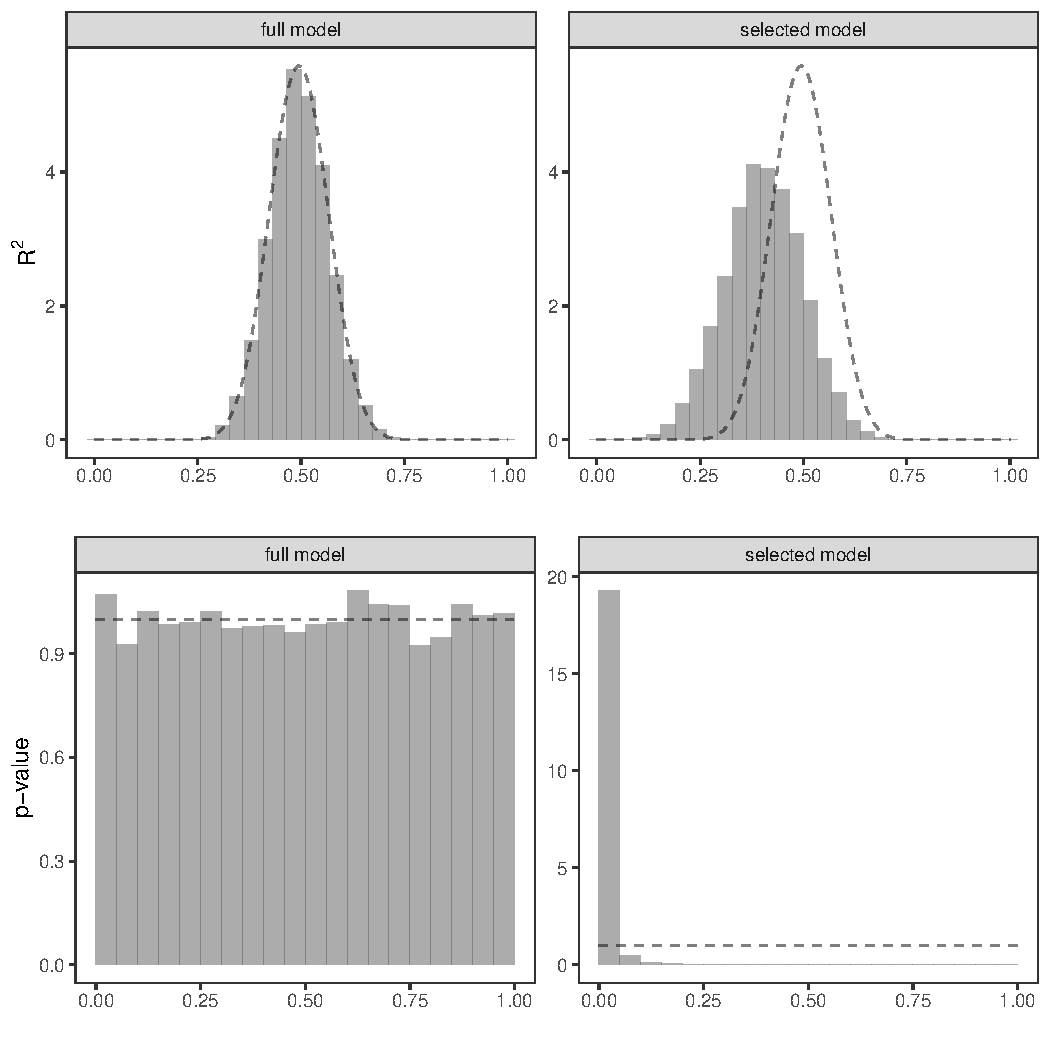
\includegraphics[width =  \textwidth]{figures/freedman_simulation_ggplot.pdf}
\caption{Freedman's simulation. The first row shows the histograms of the $R^2$s, and the second row shows the histograms of the $p$-values in testing that all coefficients are 0. The first column corresponds to the full model without testing, and the second column corresponds to the selected model with testing.
}\label{fig::freedman-simulation}
\end{figure}


Figure \ref{fig::freedman-simulation} shows the results from Freedman's simulation setting with $n=100$ and $p=50$, over $1000$ replications. The \ri{R} code is in \ri{code13.1.R}. 
The $(1,1)$th subfigure shows the histogram of the $R^2$, which centers around $0.5$. 
This can be easily explained by the exact distribution of $R^{2}$ proved in Corollary \ref{coro::dist-r2}: 
\[
R^{2}\sim\textup{Beta}\left(\frac{p-1}{2},\frac{n-p}{2}\right),
\]
with the density shown in the $(1,1)$th and $(1,2)$th subfigure of Figure \ref{fig::freedman-simulation}. The beta distribution above has mean
\[
E(R^{2})=\frac{\frac{p-1}{2}}{\frac{p-1}{2}+\frac{n-p}{2}}=\frac{p-1}{n-1}
\]
 and variance
\begin{eqnarray*}
\var(R^{2}) 
&=& \frac{\frac{p-1}{2}\times\frac{n-p}{2}}{\left(\frac{p-1}{2}+\frac{n-p}{2}\right)^{2}\left(\frac{p-1}{2}+\frac{n-p}{2}+1\right)} \\
&=&\frac{2(p-1)(n-p)}{(n-1)^{2}(n+1)}.
\end{eqnarray*}
When $p/n\rightarrow0$, we have 
\[
E(R^{2})\rightarrow0,\quad\var(R^{2})\rightarrow0,
\]
so Markov's inequality implies that $R^{2}\rightarrow0$ in probability.
However, when $p/n\rightarrow\gamma\in(0,1)$, we have 
\[
E(R^{2})\rightarrow\gamma,\quad\var(R^{2})\rightarrow0,
\]
so Markov's inequality implies that $R^{2}\rightarrow\gamma$ in probability.
This means that when $p$ has the same order as $n$, the sample
$R^{2}$ is close to the ratio $p/n$ even though there is no association
between the covariates and the outcome in the true data-generating
process. In Freedman's simulation, $\gamma=0.5$ so $R^{2}$ is close
to $0.5$. 


The $(1,2)$th subfigure shows the histogram of the $R^2$ based on a model selection first step by dropping all covariates with $p$-values larger than 0.25. The $R^2$ in the $(1,2)$th subfigure are slightly smaller but still centered around $0.37$. The joint $F$ test based on the selected model does not generate uniform $p$-values in the $(2,2)$th subfigure, in contrast to the uniform $p$-values in the $(2,1)$th subfigure. With a model selection step, statistical inference becomes much more complicated. This is a topic called {\it selective inference} which is beyond the scope of this book. 




The above simulation and calculation give an important warning: we cannot
over-interpret the sample $R^{2}$ since it can be too optimistic
about model fitting. In many empirical research, $R^{2}$ is at most
$0.1$ with a large number of covariates, making us wonder whether those researchers are just chasing the noise rather than the signal. So we do not trust $R^{2}$ as a model-fitting measure with a
large number of covariates. In general, $R^2$ cannot avoid overfitting, and we must modify it in model selection. 





\section{Variance inflation factor}


The following theorem quantifies the potential problem of including too many covariates in OLS. 

\begin{theorem}
\label{theorem:varianceinflationfactor}
Consider a fixed design matrix $X$.
Let $\hat{\beta}_{j}$ be the coefficient of $X_{j}$ of the OLS fit
of $Y$ on $(1_{n},X_{1},\ldots,X_{q} ) $ with $q \leq p$. Under the
model $y_{i}=f(x_{i})+\varepsilon_{i}$ with an unknown $f(\cdot)$ and the $\varepsilon_{i}$'s
uncorrelated with mean zero and variance $\sigma^{2}$, the variance
of $\hat{\beta}_{j}$ equals  
\[
\var(\hat{\beta}_{j})=\frac{\sigma^{2}}{\sumn(x_{ij}-\bar{x}_{j})^{2}}\times\frac{1}{1-R_{j}^{2}},
\]
where $R_{j}^{2}$ is the sample $R^{2}$ from the OLS fit of $X_{j}$
on $1_{n}$ and all other covariates. 
\end{theorem}



Theorem \ref{theorem:varianceinflationfactor} does not even assume that the true mean function is linear. It 
states that the variance
of $\hat{\beta}_{j}$ has two multiplicative components. If we run
a short regression of $Y$ on $1_{n}$ and $X_{j} = (x_{1j}, \ldots, x_{nj})^{\T}$, the coefficient equals
\[
\tilde{\beta}_{j}=\frac{\sumn(x_{ij}-\bar{x}_{j})y_{i}}{\sumn(x_{ij}-\bar{x}_{j})^{2}}
\]
where $\bar{x}_{j} = n^{-1} \sumn x_{ij}$. It
has variance
\begin{eqnarray*}
\var(\tilde{\beta}_{j}) &=& \var\left\{ \frac{\sumn(x_{ij}-\bar{x}_{j})y_{i}}{\sumn(x_{ij}-\bar{x}_{j})^{2}}\right\} \\
&=&\frac{\sumn(x_{ij}-\bar{x}_{j})^{2}\sigma^{2}}{\left\{ \sumn(x_{ij}-\bar{x}_{j})^{2}\right\} ^{2}} \\
&=&\frac{\sigma^{2}}{\sumn(x_{ij}-\bar{x}_{j})^{2}}.
\end{eqnarray*}
So the first component is the variance of the OLS coefficient in the
short regression. The second component $1/(1-R_{j}^{2})$ is called
the variance inflation factor (VIF). The VIF indeed inflates the variance
of $\tilde{\beta}_{j}$, and the more covariates are added into the
long regression, the larger the variance inflation factor is. 
In \ri{R}, the \ri{car} package provides the function \ri{vif} to compute the VIF for each covariate. 

The proof of Theorem \ref{theorem:varianceinflationfactor} below is based
on the FWL theorem. 



\begin{myproof}{Theorem}{\ref{theorem:varianceinflationfactor}}
Let $\tilde{X}_{j} = (\tilde{x}_{1j}, \ldots, \tilde{x}_{nj})^{\T}$ be the residual vector from the OLS fit of $X_{j}$
on $1_{n}$ and other covariates, which have a sample mean of zero. The FWL
theorem implies that 
\[
\hat{\beta}_{j}=\frac{\sumn\tilde{x}_{ij}y_{i}}{\sumn\tilde{x}_{ij}^{2}}
\]
which has variance
\begin{equation}\label{eq::vif-variance1}
\var(\hat{\beta}_{j})=\frac{\sumn\tilde{x}_{ij}^{2}\sigma^{2}}{\left\{ \sumn\tilde{x}_{ij}^{2}\right\} ^{2}}=\frac{\sigma^{2}}{\sumn\tilde{x}_{ij}^{2}}.
\end{equation}
Because $\sumn\tilde{x}_{ij}^{2}$ is the residual sum of squares
from the OLS of $X_{j}$ on $1_{n}$ and other covariates, it is
related to $R_{j}^{2}$ via
\[
R_{j}^{2}=1-\frac{\sumn\tilde{x}_{ij}^{2}}{\sumn(x_{ij}-\bar{x}_{j})^{2}}
\]
or, equivalently,
\begin{equation}\label{eq::vif-variance2}
\sumn\tilde{x}_{ij}^{2}=(1-R_{j}^{2})\sumn(x_{ij}-\bar{x}_{j})^{2}.
\end{equation}
Combining \eqref{eq::vif-variance1} and \eqref{eq::vif-variance2} gives Theorem \ref{theorem:varianceinflationfactor}. 
\end{myproof}





\section{Bias-variance trade-off}

Theorem \ref{theorem:varianceinflationfactor} characterizes the variance
of the OLS coefficient, but it does not characterize its bias. In
general,   a more complex model is closer to
the true mean function $f(x_i)$, and can then reduce the bias of approximating the mean function.
However, Theorem \ref{theorem:varianceinflationfactor} implies that a more complex model results in larger variances of the OLS
coefficients. So we face a bias-variance trade-off. 



Consider a simple case where the true data-generating process is linear:
\begin{equation}
y_{i}=\beta_{1}+\beta_{2}x_{i1}+\cdots+\beta_{s-1}x_{is}+\varepsilon_{i} . \label{eq:correct-model}
\end{equation}
Ideally, we want
to use the model (\ref{eq:correct-model}) with exactly $s$ covariates. In practice, we may not know which covariates to include in the OLS. 
If we underfit the data using a short regression with $q<s$: 
\begin{equation}
y_{i}=\tilde{\beta}_{1}+\tilde{\beta}_{2}x_{i1}+\cdots+\tilde{\beta}_{q-1}x_{iq}+\tilde{\varepsilon}_{i},\qquad(i=1,\ldots,n)\label{eq:underfitted-model}
\end{equation}
then the OLS coefficients are biased. If we increase the complexity of
the model to overfit the data using a long regression with $p>s$: 
\begin{equation}
y_{i}=\hat{\beta}_{1}+\hat{\beta}_{2}x_{i1}+\cdots+\hat{\beta}_{p-1}x_{ip}+\hat{\varepsilon}_{i},\qquad(i=1,\ldots,n)\label{eq:overfitted-model}
\end{equation}
then the OLS coefficients are unbiased. Theorem \ref{theorem:varianceinflationfactor},
however, shows that the OLS coefficients from the under-fitted model
(\ref{eq:underfitted-model}) have smaller variances than those from
the overfitted model (\ref{eq:overfitted-model}). 




\begin{example}\label{example::bias-variance-tradeoff}
In general, we have a sequence of models with increasing complexity.
For simplicity, we consider nested models containing $1_{n}$ and covariates
\[
\left\{ X_{1}\right\} \subset\left\{ X_{1},X_{2}\right\} \subset\cdots\subset\left\{ X_{1},\ldots,X_{p}\right\}
\]
in the following simulation setting. The true linear model is $y_i=x_i^{\T} \beta + \N(0,1)$ with $p=40$ but only the first 10 covariates have non-zero coefficients 1 and all other covariates have coefficients 0. 
We generate two datasets: both have sample size $n=200$, all covariates have IID $\N(0,1)$ entries, and the error terms are IID.
We use the first dataset to fit the OLS and thus call it the {\it training dataset}. We use the second dataset to assess the performance of the fitted OLS from the training dataset, and thus call it the {\it testing dataset}\footnote{Splitting a dataset into the training and testing datasets is a standard tool to assess the out-of-sample performance of proposed methods. It is important in statistics and machine learning.}.
Figure \ref{fig::bias-variance-tradeoff-linearmodel} plots the residual sum of squares against the number of covariates in the training and testing datasets. By definition of OLS, the residual sum of squares decreases with the number of covariates in the training dataset, but it first decreases and then increases in the testing dataset with minimum value attained at $10$, the number of covariates in the true data generating process. 
\end{example}


 
\begin{figure}[th]
\centering 
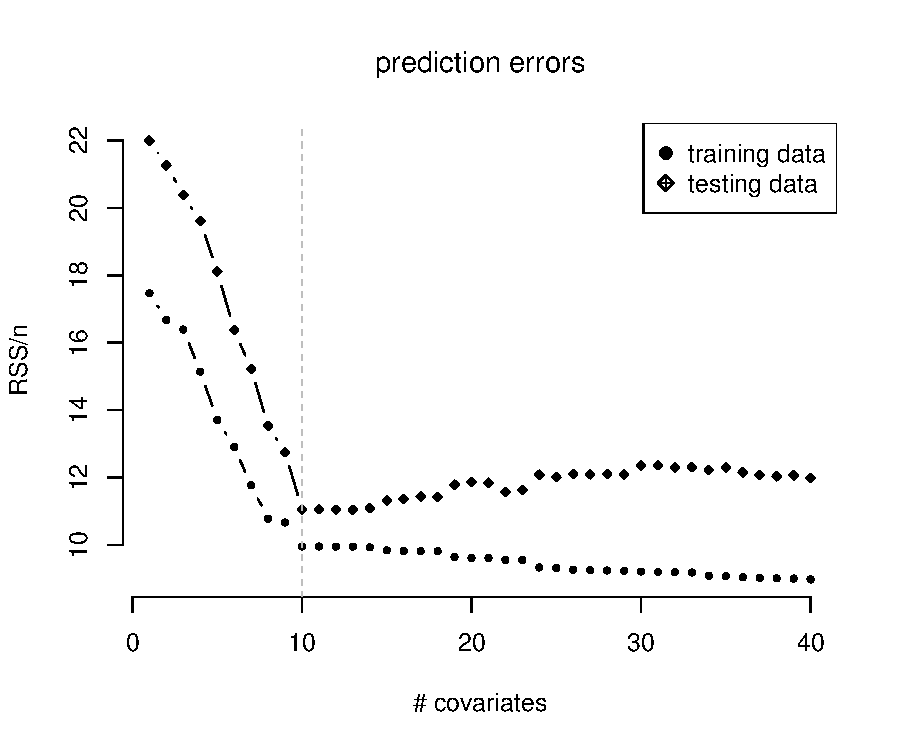
\includegraphics[width = 0.8\textwidth]{figures/training_testing_error.pdf}
\caption{Training and testing errors: linear mean function}\label{fig::bias-variance-tradeoff-linearmodel}
\end{figure}



The following example has a nonlinear true mean function but still uses OLS with polynomials of covariates to approximate the truth\footnote{A celebrated theorem due to Weierstrass states that on a bounded interval, any continuous function can be approximated arbitrarily well by a polynomial function. Here is the mathematical statement of Weierstrass's theorem.  
Suppose $f$ is a continuous function defined on the interval $[a, b]$. For every $\varepsilon  > 0$, there exists a polynomial $p$ such that for all $x \in [a, b]$, we have $|f(x) - p(x) | < \varepsilon $.}. 




\begin{example}
The true nonlinear model is $y_i  = \sin(2\pi x_i) + \N(0,1)$ with the $x_i$'s equally spaced in $[0,1]$ and the error terms are IID. The training and testing datasets both have sample sizes $n=200$. Figure \ref{fig::bias-variance-tradeoff-linearmodel-poly} plots the residual sum of squares against the order of the polynomial in the OLS fit
$$
y_i = \sum_{j=0}^{p-1} \beta_j x_i^j + \varepsilon_i.
$$
By the definition of OLS, the residual sum of squares decreases with the order of polynomials in the training dataset, but it achieves the minimum near $p=5$ in the testing dataset. We can show that the residual sum of squares decreases to zero with $p=n$ in the training dataset; see Problem \ref{hw12::perfect-polynomial}. However, it is larger than that under $p=5$ in the testing dataset. 
\end{example}


\begin{figure}[th]
\centering 
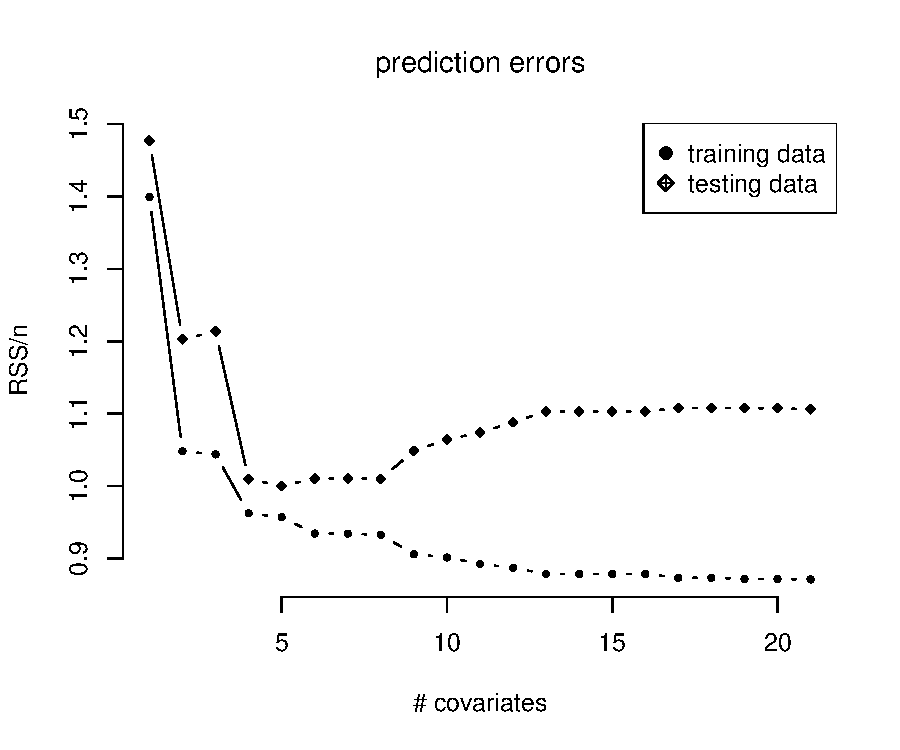
\includegraphics[width = 0.8 \textwidth]{figures/training_testing_error_poly.pdf}
\caption{Training and testing errors: nonlinear mean function}\label{fig::bias-variance-tradeoff-linearmodel-poly}
\end{figure}
 

The \ri{R} code for Figures \ref{fig::bias-variance-tradeoff-linearmodel} and \ref{fig::bias-variance-tradeoff-linearmodel-poly} is in \ri{code13.3.R}. 



\section{Model selection criteria}

With a large number of covariates $X_{1},\ldots,X_{\overline{p}}$, we want to
select a model that has the best performance for prediction. In total,
we have $2^{\overline{p}}$ possible models. Which one is the best? What is the
criterion for the best model? Practitioners often use the linear model for multiple purposes. A dominant criterion is the prediction performance of the linear model in a new dataset \citep{yu2020veridical}.
However, we do not have the new dataset yet in the statistical modeling stage. So we need to find criteria that are good proxies for the prediction performance. 



\subsection{RSS, $R^{2}$ and adjusted $R^{2}$}

The first obvious criterion is the \textsc{rss}, which, however, is not a good criterion because it favors the largest model. 
The sample $R^{2}$ has the same problem of favoring the largest model.
Most model selection criteria are in some sense modifications of \textsc{rss} or $R^2$.

 
The adjusted $R^{2}$ takes into account the complexity of the model:
\begin{align*}
\bar{R}^{2} & =1-\frac{n-1}{n-p}(1-R^{2})\\
 & =1-\frac{\sumn(y_{i}-\hat{y}_{i})^{2}/(n-p)}{\sumn(y_{i}-\bar{y})^{2}/(n-1)}\\
 & =1-\frac{\hat{\sigma}^{2}}{\hat{\sigma}_{y}^{2}}.
\end{align*}
So based on $\bar{R}^{2}$, the best model has the smallest $\hat{\sigma}^{2}$,
the estimator for the variance of the error term in the Gauss--Markov
model. The following theorem shows that $\bar{R}^{2}$ is closely related to the $F$ statistic in
testing two nested Normal linear models. 


\begin{theorem}
\label{theorem:Fstat-adjustedR2} 
Consider the setting of Chapter \ref{sec::fwl-anova}.
Test two nested Normal linear
models:
\[
Y=X_{1}\beta_{1}+\varepsilon
\]
versus
\[
Y=X_{1}\beta_{1}+X_{2}\beta_{2}+\varepsilon,
\]
or, equivalently, test $\beta_{2}=0$. We can use the standard
$F$ statistic defined in Chapter \ref{sec::fwl-anova}, and we can also compare the adjusted $R^{2}$'s from
these two models: $\bar{R}_{1}^{2}$ and $\bar{R}_{2}^{2}$. They
are related via
\[
F>1\Longleftrightarrow\bar{R}_{1}^{2}<\bar{R}_{2}^{2}.
\]
\end{theorem}


I leave the proof of the theorem as Problem \ref{hw12::f-r2}. 
From Theorem \ref{theorem:Fstat-adjustedR2}, $\bar{R}^{2}$ does not necessarily favor the largest model. However, $\bar{R}^{2}$ still
favors unnecessarily large models compared with the usual
hypothesis testing based on the Normal linear model because the mean of $F$ is approximately $1$, but the upper
quantile of $F$ is much larger than $1$ (for example, the 95\% quantile of $F_{1,n-p}$ is larger than 3.8, and the 95\% quantile of $F_{2,n-p}$ is larger than 2.9). 



\subsection{Information criteria}


Taking into account the model complexity, we can find the model with the smallest \textsc{aic} or \textsc{bic}, defined as
\[
\textsc{aic}=n\log\frac{\textsc{rss}}{n}+2p
\]
and
\[
\textsc{bic}=n\log\frac{\textsc{rss}}{n}+p\log n,
\]
with full names
``Akaike's information criterion '' and 
``Bayes information criterion.''

\textsc{aic} and \textsc{bic} are both monotone functions of the \textsc{rss} penalized by the number of parameters $p$ in the model. The penalty in \textsc{bic} is larger so it favors smaller models than \textsc{aic}. \citet{shao1997asymptotic}'s results suggested that \textsc{bic} can consistently select the true model if the linear model is correctly specified, but \textsc{aic} can select the model that minimizes the prediction error if the linear model is misspecified. In most statistical practice, the linear model assumption cannot be justified, so we recommend using \textsc{aic}. 




\subsection{Cross-validation (CV)}

The first choice is the leave-one-out cross-validation based on the predicted residual: 
\begin{equation}
\label{eq::press-stat}
\textsc{press}=\sumn\hat{\varepsilon}_{[-i]}^{2}=\sumn\frac{\hat{\varepsilon}_i^{2}}{(1-h_{ii})^{2}}
\end{equation}
which is called the predicted residual error sum of squares (PRESS)
statistic. 

Because the average value of $h_{ii}$ is $n^{-1}\sumn h_{ii}=p/n$,
we can approximate PRESS by the generalized cross-validation (GCV)
criterion:
\[
\textsc{gcv}=\sumn\frac{\hat{\varepsilon}_i^{2}}{(1-p/n)^{2}}=\textsc{rss}\times\left(1-\frac{p}{n}\right)^{-2}.
\]
When $p/n\approx0$, we have\footnote{The approximation is due to the Taylor expansion $\log(1+x) = x - x^2/2 + x^3/3 - \cdots \approx x$.}
\[
\log\textsc{gcv}=\log\textsc{rss}-2\log\left(1-\frac{p}{n}\right)\approx\log\textsc{rss}+\frac{2p}{n}=\textsc{aic}/n+\log n,
\]
so GCV is approximately equivalent to AIC with small $p/n$. With large $p/n$, they may have large differences. 

GCV is not crucial for OLS because it is easy to compute PRESS.
However, it is much more useful in other models where
we need to fit the data $n$ times to compute PRESS. 
For a general model without simple leave-one-out formulas, it is computationally intensive to obtain PRESS. The
$K$-fold cross-validation ($K$-CV) is computationally more attractive. The best model has the smallest $K$-CV, computed as follows:
\begin{enumerate}
\item randomly shuffle the observations;
\item split the data into $K$ folds;
\item for each fold $k$, use all other folds as the training data, and
compute the predicted errors on fold $k$ $(k=1,\ldots, K)$;
\item aggregate the prediction errors across $K$ folds, denoted by $K$-CV.
\end{enumerate}

When $K  = 3$, we split the data into $3$ folds. Run OLS to obtain a fitted function with folds $2,3$ and use it to predict on fold 1, yielding prediction error $r_1$;  run OLS with folds $1,3$ and predict on fold $2$,  yielding prediction error $r_2$; run OLS with folds $1, 2$ and predict on fold $2$, yielding prediction error $r_3$. The total prediction error is $r = r_1  + r_2 + r_3$. We want to select a model that minimizes $r$. Usually, practitioners choose $K=5$ or $10$, but this can depend on the computational resource. 



\section{Best subset and forward/backward selection}

Given a model selection criterion, we can select the best model. 

For a small $\overline{p}$, we can enumerate all $2^{\overline{p}}$ models. The function \ri{regsubsets} in the \ri{R} package \ri{leaps} implements this\footnote{Note that this function uses a definition of \textsc{bic} that differs from the above definition by a constant, but this does not change the model selection result.}.
Figure \ref{fig::best-subset-selection-penn-boston} shows the results of the best subset selection in two applications, with the code in \ri{code13.4.4.R}.  


\begin{figure}[ht]
\centering 
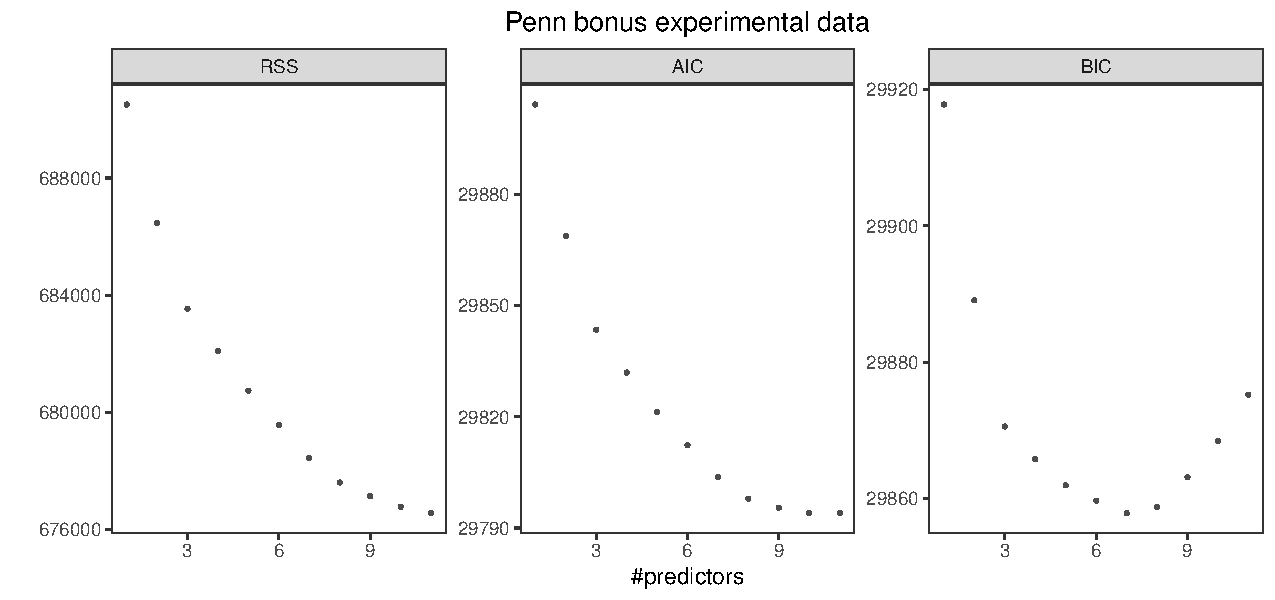
\includegraphics[width =  \textwidth]{figures/bestsubsetpenn}
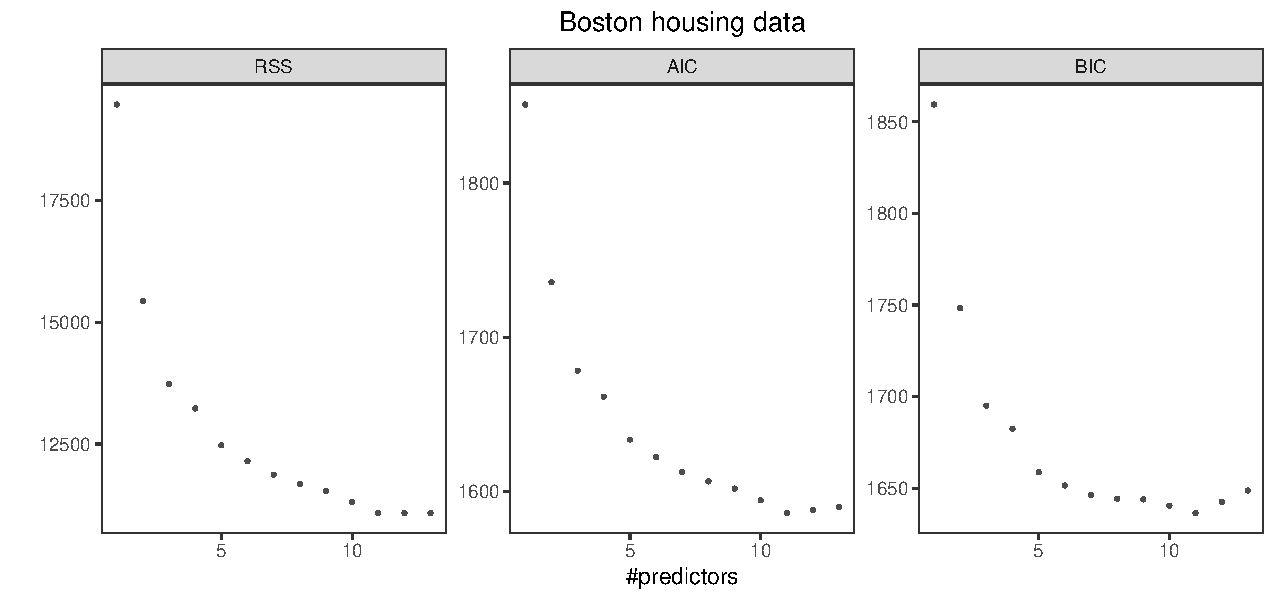
\includegraphics[width = \textwidth]{figures/bestsubsetbostonhousing} 
\caption{Best subset selection}\label{fig::best-subset-selection-penn-boston}
\end{figure}

For large $\overline{p}$, we can use forward or backward regressions. 
Forward regression starts with a model with only the intercept. In step one, it finds the best covariate among the $\overline{p}$ candidates based on the prespecified criterion. In step two, it keeps this covariate in the model and finds the next best covariate among the remaining $\overline{p} - 1$ candidates. It proceeds by adding the next best covariate one by one. 


The backward regression does the opposite. It starts with the full model with all $\overline{p}$ covariates. In step one, it drops the worst covariate among the $\overline{p}$ candidates based on the prespecified criterion. In step two, it drops the next worst covariate among the remaining $\overline{p} - 1$ candidates. It proceeds by dropping the next worst covariate one by one. 


Both methods generate a sequence of models, and select the best one based on the prespecified criterion. Forward regression works in the case with $p\geq n$ but it stops at step $n-1$; backward regression works only in the case with $p<n.$
The functions
\ri{step} or \ri{stepAIC} in the \ri{MASS} package implement these. 

 

\section{Homework problems}


\paragraph{Inflation and deflation of the estimated variance}\label{hw12::inf-def-est-var}

This problem extends Theorem \ref{theorem:varianceinflationfactor} to the estimated variance. 

The covariate matrix $X$ has columns $1_n, X_1, \ldots, X_p$. 
Compare the coefficient of $X_1$ in the following long and short regressions:
$$
Y = \hat{\beta}_0 1_n  + \hat{\beta}_1 X_1 + \cdots + \hat{\beta}_p X_p  +\hat \varepsilon,
$$
and 
$$ 
Y =\tilde{\beta}_0 1_n  +  \tilde{\beta}_1 X_1 + \cdots + \tilde{\beta}_q  X_q   +\tilde \varepsilon,
$$
where $q < p$. Under the condition in Theorem \ref{theorem:varianceinflationfactor}, 
$$  \frac { \var( \hat{\beta}_1 ) }{  \var( \tilde{\beta}_1 ) }
 = \frac{  1- R^2_{X_1.X_2\cdots X_q}  }{  1- R^2_{X_1.X_2\cdots X_p}   } \geq 1 ,
$$
recalling that $R^2_{U.V}$ denotes the $R^2$ of $U$ on $V$. 
Now we compare the corresponding estimated variances $\hat \var( \hat{\beta}_1 )$ and $\tilde \var( \tilde{\beta}_1 )$ based on homoskedasticity. 

\begin{enumerate}
\item
Show that
$$
\frac{\hat \var( \hat{\beta}_1 )}{  \tilde \var( \tilde{\beta}_1 ) }
=   \frac{   1 - R^2_{Y.X_1\cdots X_p}  }{  1 - R^2_{Y.X_1\cdots X_q}  } \times  \frac{  1- R^2_{X_1.X_2\cdots X_q}  }{  1- R^2_{X_1.X_2\cdots X_p}   }  \times \frac{n-q - 1}{n-p - 1}    . 
$$


\item
Using the definition of the partial $R^2$ in Problem \ref{hw09::partial-R2}, show that
$$
\frac{\hat \var( \hat{\beta}_1 )}{  \tilde \var( \tilde{\beta}_1 ) }
=    \frac{   1 - R^2_{Y.X_{q+1} \cdots X_p  \mid  X_1\cdots X_q}  }{  1 - R^2_{ X_1.X_{q+1}\cdots X_p \mid  X_2\ldots X_q}  }  
\times  \frac{n-q - 1}{n-p - 1} .
$$
\end{enumerate}









Remark: The first result shows that the ratio of the estimated variances has three factors: the first one corresponds to the $R^2$'s of the outcome on the covariates,  the second one is identical to the one for the ratio of the true variances, and the third one corresponds to the degrees of freedom correction. The first factor deflates the estimated variance since the $R^2$ increases with more covariates included in the regression, and the second and the third factors inflate the estimated variance. Overall, whether adding more covariates inflate or deflate the estimated variance depends on the interplay of the three factors. The answer is not definite as Theorem \ref{theorem:varianceinflationfactor}. 


The variance inflation result in Theorem \ref{theorem:varianceinflationfactor} sometimes causes confusion. It only concerns the variance. When we view some covariates as random, then the bias term can also contribute to the variance of the OLS estimator. In this case, we should interpret Theorem \ref{theorem:varianceinflationfactor} with caution. See \citet{ding2019two} for a related discussion. 


 


\paragraph{Inflation and deflation of the variance under heteroskedasticity}\label{hw12::inf-def-heteroskedasticity}

Relax the condition in Theorem \ref{theorem:varianceinflationfactor}  as $\var(\varepsilon_i) = \sigma_i^2$ with possibly different variances.  Give a counterexample in which the variance decreases with more covariates included in the regression. 



\paragraph{Equivalence of $F$ and $\bar{R}^{2}$}\label{hw12::f-r2}

Prove Theorem \ref{theorem:Fstat-adjustedR2}. 


\paragraph{Using \textsc{press} to construct an unbiased estimator for $\sigma^2$}\label{hw12::press-unbiased-sigma2}


Prove that 
$$
\hat{\sigma}^{2}_{\textsc{press}} 
= 
\frac{  \textsc{press}  }{ \sumn (1-h_{ii})^{-1}   }
$$
is unbiased for $\sigma^2$ under the Gauss--Markov model in Assumption \ref{assume::gm-model}, recalling $\textsc{press} $ in \eqref{eq::press-stat} and the leverage score $h_{ii}$ of unit $i$. 


Remark: Theorem \ref{thm:varianceestOLS} shows that $\hat{\sigma}^{2}=\textsc{rss}/(n-p)$ is unbiased for $\sigma^2$ under the Gauss--Markov model. 
\textsc{rss} is the ``in-sample'' residual sum of squares, whereas \textsc{press} is the ``leave-one-out'' residual sum of squares. 
The estimator $\hat{\sigma}^{2}$ is standard, whereas $\hat{\sigma}^{2}_{\textsc{press}} $ appeared in \citet{shen2023algebraic}. 




\paragraph{Simulation with misspecified linear models}

Replicate the simulation in Example \ref{example::bias-variance-tradeoff} with correlated covariates and an outcome model with quadratic terms of covariates. 

\paragraph{Best subset selection in \ri{lalonde} data}

Produce the figure similar to the ones in Figure \ref{fig::best-subset-selection-penn-boston} based on the \ri{lalonde} data in the \ri{Matching} package. Report the selected model based on \textsc{aic}, \textsc{bic}, \textsc{press}, and \textsc{gcv}. 


 \paragraph{Perfect polynomial}\label{hw12::perfect-polynomial}
 
Prove that given distinct $x_i \ (i=1, \ldots, n)$ within $[0,1]$ and any $y_i\ (i=1, \ldots, n)$, we can always find an $n$th order polynomial 
$$
p_n(x) = \sum_{j=0}^{n-1} b_j x^j
$$ 
such that 
$$
p_n(x_i) = y_i, \quad  (i=1, \ldots, n).
$$

Hint: Use the formula in \eqref{eq::det-Vandermonde}. 
 
 
 
 

